\documentclass[10pt]{beamer}



\usepackage{multirow}


% Perintah untuk membuat huruf tercetak miring. (alias)
\newcommand{\f}[1]{\textit{#1}}
% Perintah untuk huruf tercetak tebal dan miring.
\newcommand{\bi}[1]{\textbf{\textit{#1}}}
% Perintah untuk huruf tercetak tebal.
\newcommand{\bo}[1]{\textbf{#1}}
% Perintah untuk mencetak tebal di persamaan matematis
\newcommand{\m}[1]{\boldmath{ \( #1 \)}}
\newcommand{\mc}[1]{\boldmath{ \[ #1 \]}}
% Perintah untuk cetak in-line code
\newcommand{\code}[1]{\texttt{#1}}


\usepackage[natbibapa]{apacite}
\bibliographystyle{apacite}
\AtBeginDocument{
	\renewcommand{\refname}{\bibname}
	\renewcommand{\BBAA}{\&}
	\renewcommand{\BBAB}{dan}
	\renewcommand{\BRetrievedFrom}{Diakses dari }
	\renewcommand{\BRetrieved}[1]{Diakses pada tanggal {#1}, dari\ }
}

\AtBeginSection[]
{
  \begin{frame}
    \frametitle{Table of Contents}
    \tableofcontents[currentsection]
  \end{frame}
}



\title{Aplikasi \f{Bidirectional Encoder Representations from Transformers} untuk Pemeringkatan Teks Bahasa Indonesia}


\author{Carles Octavianus \\ Dosen Pembimbing: Sarini Abdullah S.Si., M.Stats., Ph.D.}


\date{3 Januari, 2024}

\logo{
\includegraphics[height=1cm]{assets/pics/makara_kuning.png}}


\begin{document}

\frame{\titlepage}




\begin{frame}
    \frametitle{Daftar Isi}
    \tableofcontents
\end{frame}


\section{Pendahuluan}
\begin{frame}
    \frametitle{Pendahuluan}

\begin{enumerate}
    \item Peningkatan jumlah data teks digital membuat manusia kesulitan dalam memproses informasi secara efektif dan efisien.
    \item Tahap pertama dalam memproses informasi dari data teks adalah melakukan penyimpanan data teks dengan efisien.
    \item Diperlukan mekanisme untuk mengembalikan teks yang relevan dari kumpulan data teks tersebut. Mekanisme pengembalian teks menjadi semakin penting dengan peningkatan jumlah data teks.
\end{enumerate}
\end{frame}

\begin{frame}
    \frametitle{Pendahuluan}
    \begin{enumerate}
        \setcounter{enumi}{2}
        \item Pemeringkatan teks adalah salah satu mekanisme untuk mengembalikan teks yang relevan.
        \item Tujuan dari pemeringkatan teks adalah menghasilkan daftar teks yang terurut berdasarkan relevansinya terhadap permintaan pengguna.
    \end{enumerate}
\end{frame}

\frametitle{Alur Pemeringkatan Teks Klasik}
\begin{frame}
    \begin{figure}
        \centering
        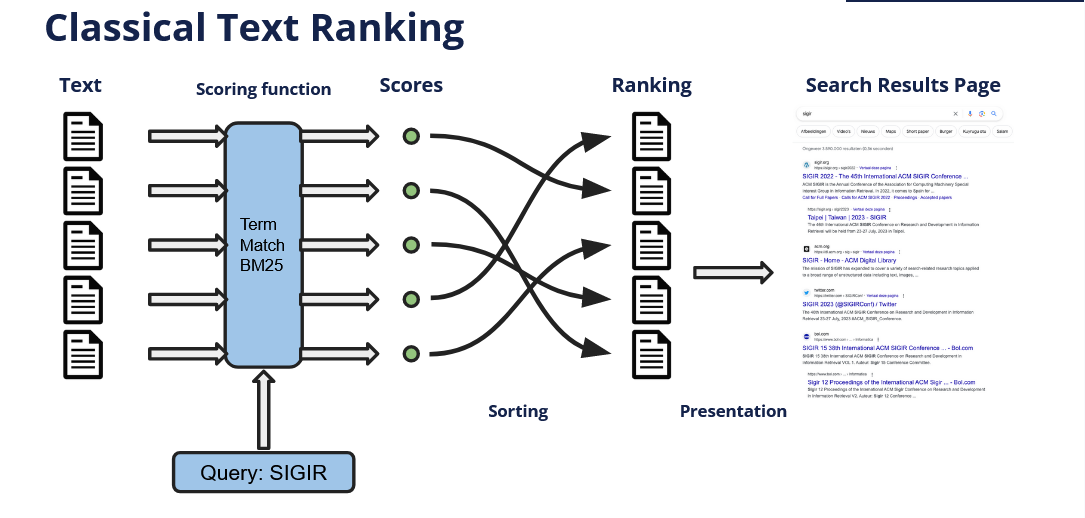
\includegraphics[width=1\textwidth]{assets/pics/classical-IR.png}
    \end{figure}
\end{frame}

\begin{frame}{\f{Vocabulary Mismatch}}
    \begin{enumerate}
        \item Kueri \code{apa makanan terenak di Indonesia}, dan teks \code{hidangan terlezat di nusantara adalah rendang} tentunya akan mendapatkan skor yang rendah bila menggunakan fungsi skoring kecocokan antara kata-kata pada kueri dan teks.
        \item Hal ini diatasi dengan penggunaan fungsi skoring berbasis \f{deep learning}.
    \end{enumerate}
\end{frame}

\begin{frame}
    \frametitle{Alur Pemeringkatan Teks dengan \f{Deep Learning}}
    \begin{figure}
        \centering
        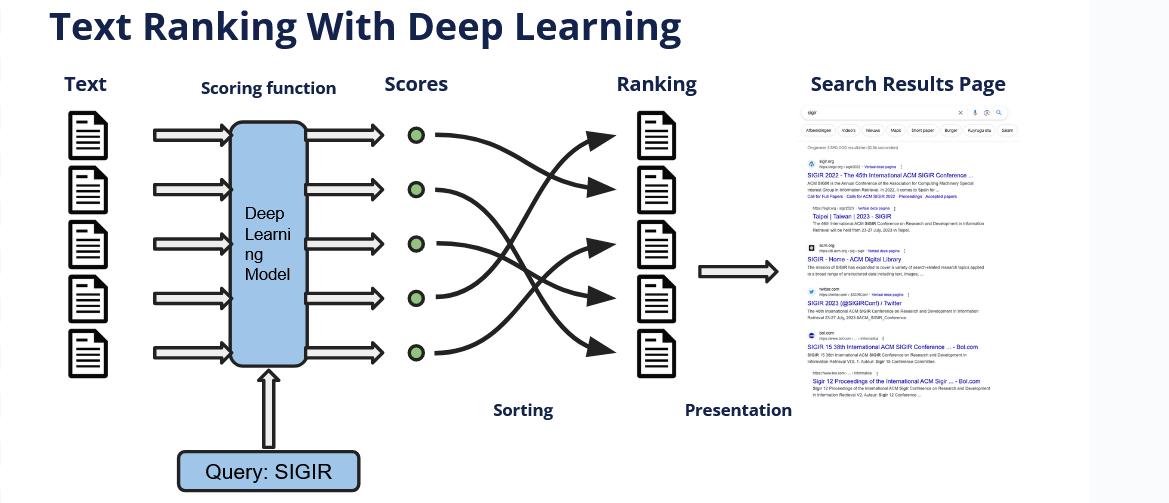
\includegraphics[width=1\textwidth]{assets/pics/DL-IR.png}
    \end{figure}
\end{frame}

\begin{frame}
    \frametitle{BERT}
    \begin{enumerate}
        \item Model \f{Bidirectional Encoder Representations from Transformers} (BERT) adalah model pra-latih \f{deep learning} yang dikembangkan oleh \cite{bertori} untuk permasalahan bahasa alami. BERT memetakan kata-kata pada kalimat menjadi representasi vektor yang kontekstual.
        \item BERT telah menjadi \f{state-of-the-art} untuk berbagai permasalahan pemrosesan bahasa alami seperti \f{question answering}, \f{named entity recognition}, \f{sentiment analysis}, dan pemeringkatan teks.
    \end{enumerate}
\end{frame}

\begin{frame}
    \frametitle{Websearch dengan BERT}
    \begin{figure}
        \centering
        
\includegraphics[width=1\textwidth]{assets/pics/google-bert.png}
    \end{figure}
\end{frame}

\begin{frame}
    \frametitle{Model Pemeringakatan Teks Bahasa Inggris}
    \begin{figure}
        \centering
        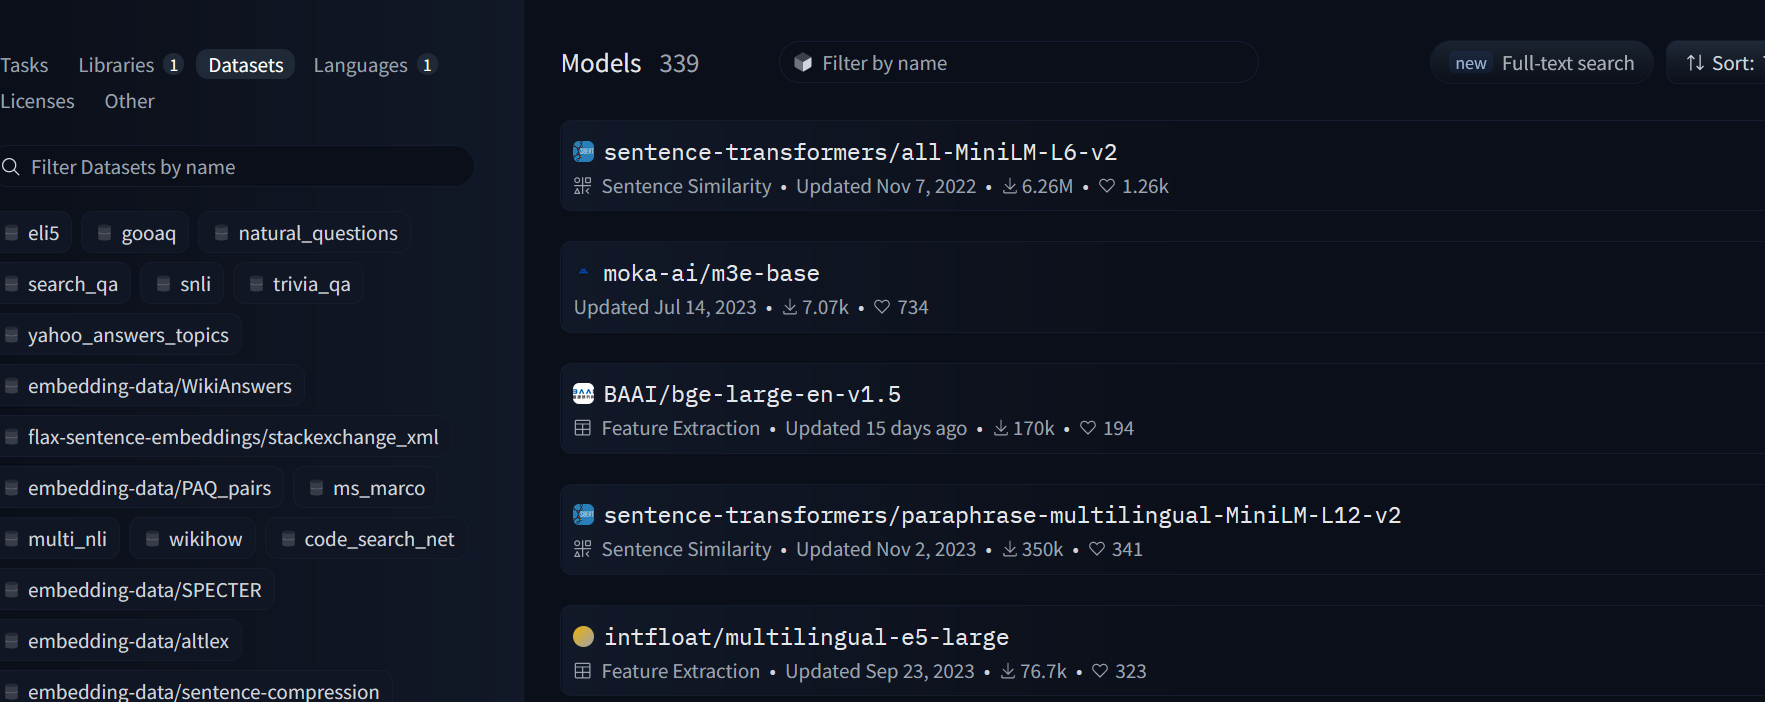
\includegraphics[width=1\textwidth]{assets/pics/EnglishNLP.png}
    \end{figure}
    Model pemeringkatan teks bahasa Inggris pada \f{HuggingFace} dengan jumlah 339 model. Variasi dan jumlah model cukup banyak, dan terdokumentasi dengan baik performa model-model tersebut.
\end{frame}

\begin{frame}
    \frametitle{Model Pemeringakatan Teks Bahasa Indonesia}
    \begin{figure}
        \centering
        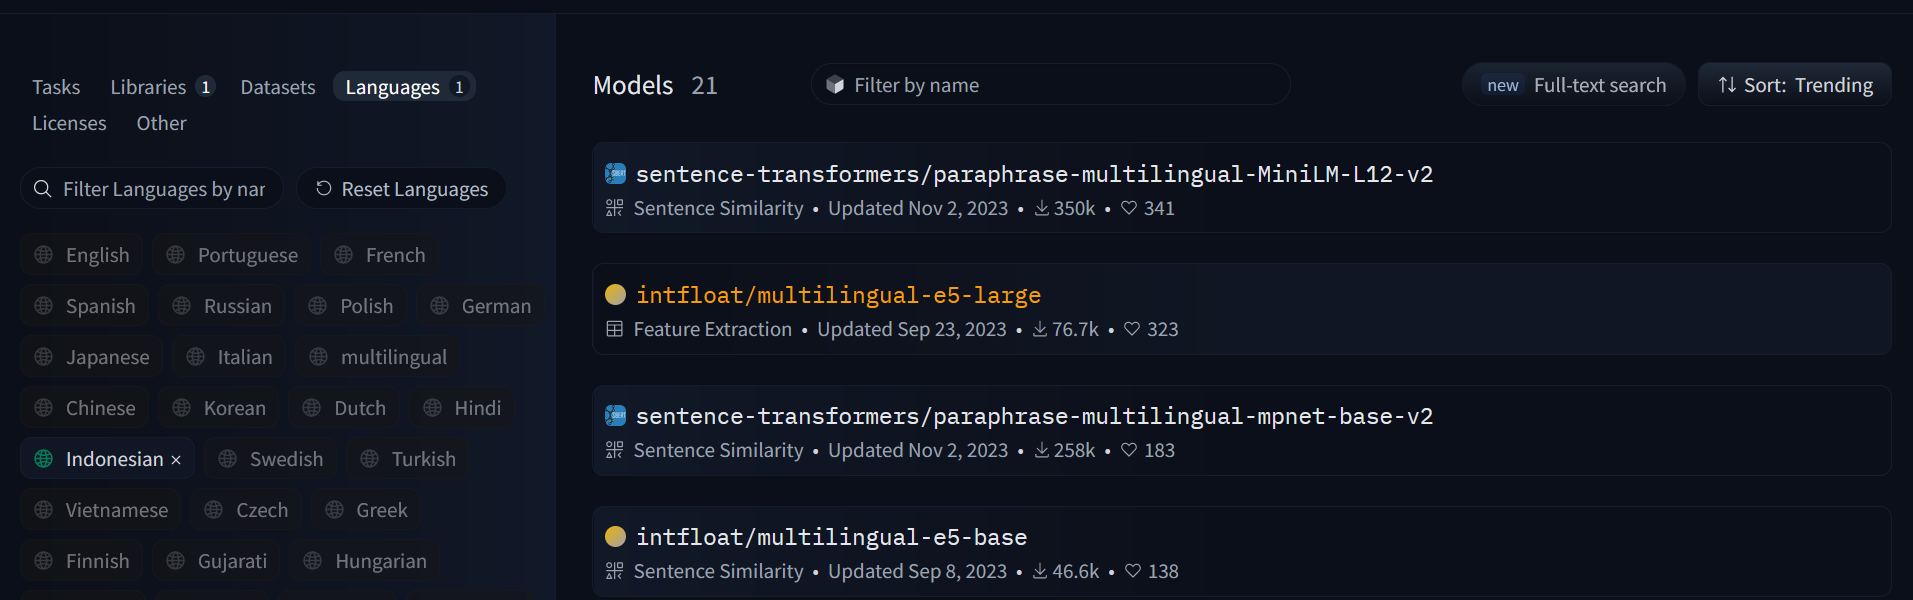
\includegraphics[width=1\textwidth]{assets/pics/IndoNLP.png}
    \end{figure}    
    Model "pemeringkatan teks" bahasa Indonesia pada \f{HuggingFace} dengan jumlah 21 model. Hanya 3 model yang bukan model multibahasa, dan dari ketiga model tersebut, tidak ada model dengan dokumentasi performa model untuk pemeringkatan teks.
\end{frame}

\begin{frame}
\frametitle{Rumusan Masalah}

\begin{enumerate}
	\item Bagaimana pengaplikasian model BERT untuk pemeringkatan teks berbahasa Indonesia?
	\item Bagaimana kinerja model BERT pada setiap \f{dataset} yang digunakan bila dibandingkan dengan model \f{baseline} BM25?
\end{enumerate}

\end{frame}

\begin{frame}
    \frametitle{Tujuan Penelitian}
    \begin{enumerate}
        \item Membangun dan melatih kembali \f{(fine tuning)} model BERT untuk pemeringkatan teks berbahasa Indonesia.
        \item Membandingkan kinerja model BERT pada setiap \f{dataset} yang digunakan bila dibandingkan dengan model \f{baseline} BM25.
    \end{enumerate}
\end{frame}

\begin{frame}
    \frametitle{Batasan Masalah}
    \begin{enumerate}
    \item \f{Dataset} yang digunakan untuk melatih kembali (\f{fine tuning}) model BERT adalah \f{dataset} mMarco \f{train set} bahasa Indonesia \citep{mmarco}.
	\item \f{Dataset} yang digunakan untuk mengukur performa model adalah \f{dataset} mMarco \f{dev set} bahasa Indonesia \citep{mmarco} untuk \f{in-domain test} serta MrTyDi \f{dev set} bahasa Indonesia \citep{mrtydi}, dan Miracl \f{dev set} bahasa Indonesia \citep{miracl} untuk \f{out-of-domain test}.
	\item Kinerja model diamati dengan metrik \f{recriprocal rank} (RR), \f{recall} (R), dan \f{normalized discounted cumulative gain} (NDCG).
    \end{enumerate}
\end{frame}
    
\section{Pemeringkatan Teks}

\begin{frame}
\frametitle{Tugas Pemeringkatan Teks}

    \begin{block}{Tugas Pemeringkatan Teks}
        Diberikan kueri $q$ dan himpunan teks terbatas $\mathcal{D}= \{d_1, d_2, ..., d_n\}$, keluaran yang diinginkan dari permasalahan ini adalah barisan teks $D_k = (d_{i_1}, d_{i_2}, ..., d_{i_k})$ yang merupakan $k$ teks yang paling relevan dengan kueri $q$.
    \end{block}
\end{frame}


\begin{frame}
    \frametitle{Bentuk Umum \f{Dataset} Uji Pemeringkatan Teks}
    \noindent\f{Dataset} Uji pada masalah pemeringkatan teks terdiri dari tiga \f{file}, yaitu \f{file} kueri, \f{file} korpus dan \f{file judgements}.
    \begin{table}[!ht]
        \centering
        \label{tab:contoh-file-korpus}
        \caption{\f{File} korpus}
        \begin{tabular}{|l|l|p{0.3\textwidth}|}
            \hline
            \textbf{\_id}    & \textbf{title}             & \textbf{text}                                                                                                 \\ \hline
            1342516\#1  & Colobothea biguttata & Larva kumbang ini biasanya mengebor ke dalam kayu dan dapat menyebabkan kerusakan $\dots$ \\ \hline
            1342517\#0  & Ichthyodes rufipes  & Ichthyodes rufipes adalah spesies kumbang tanduk panjang yang berasal dari famili Cerambycidae. Spesies ini $\dots$ \\ \hline
        \end{tabular}
    \end{table}
\end{frame}


\begin{frame}
\frametitle{Pemeringkatan Teks 3}

    \begin{table}[!ht]
        \centering
        \caption{\f{File} kueri}
        \label{tab:query-file-example}
        \begin{tabular}{|l|p{0.3\textwidth}|}
            \hline
            \textbf{\_id} & \textbf{text}                                                                 \\ \hline
            3             & Dimana James Hepburn meninggal?                                              \\ \hline
            4             & Dimana Jamie Richard Vardy lahir?                                            \\ \hline
            11            & berapakah luas pulau Flores?                                                 \\ \hline
            17            & Siapakah yang menulis Candy Candy?                                           \\ \hline
            19            & Apakah karya tulis Irma Hardisurya yang pertama?                              \\ \hline
        \end{tabular}
    \end{table}
\end{frame}


\begin{frame}
\frametitle{Pemeringkatan Teks 4}

    \begin{table}[!ht]
        \centering
        \caption{\f{File judgements}}
        \label{tab:judgements-file-example}
        \begin{tabular}{|l|l|l|}
            \hline
            \textbf{query-id} & \textbf{corpus-id} & \textbf{score} \\ \hline
            3                 & 115796\#6          & 1              \\ \hline
            3                 & 77689\#48          & 1              \\ \hline
            4                 & 1852373\#0         & 1              \\ \hline
        \end{tabular}
    \end{table}
\end{frame}

\section{Metrik Evaluasi}

\begin{frame}
    \frametitle{\f{Recall} dan Presisi}

    \begin{columns}
        \column{0.7\textwidth}
        \begin{align*}
            \text{recall}(q, D_k)\text{@k} &= \frac{\sum_{d \in D_k} \text{rel}(q, d)}{\sum_{d \in \mathcal{D}} \text{rel}(q, d)} \in [0, 1], \\ 
            \text{precision}(q, D_k)\text{@k} &= \frac{\sum_{d \in D_k} \text{rel}(q, d)}{|D_k|} \in [0, 1], \\
            \text{rel}(q, d) &= \begin{cases} 
            1 & \text{jika } r > 1 \\
            0 & \text{jika } r = 0
            \end{cases}.
        \end{align*}

        \column{0.3\textwidth}
        \begin{itemize}
            \item $q$: kueri,
            \item $D_k$: barisan $k$ teks yang dipilih oleh sistem,
            \item $r$: nilai relevansi antara kueri $q$ dengan teks $d$ dari \f{file} judgements.
        \end{itemize}
    \end{columns}
\end{frame}

\begin{frame}
    \frametitle{\f{Recall} dan Presisi}
    \begin{figure}[!ht]
        \centering
        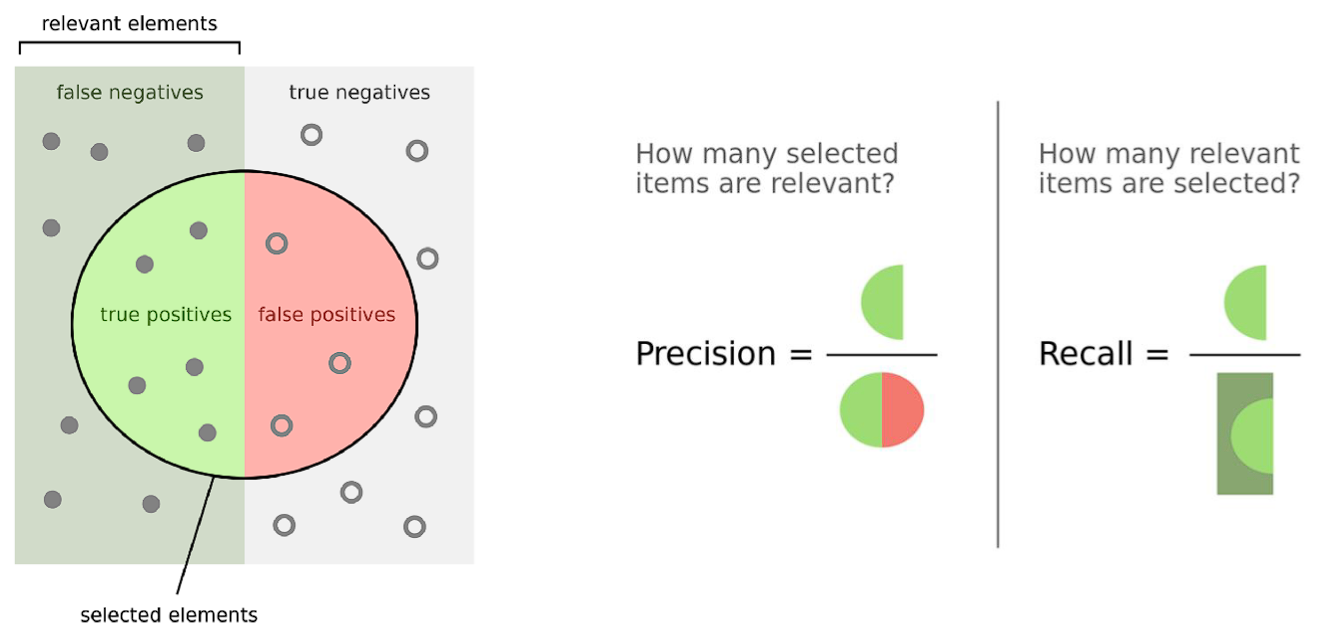
\includegraphics[width=1\textwidth]{assets/pics/recall-presisi.png}
        \caption{Ilustrasi \f{recall} dan presisi.}
        \label{fig:recall-precision}
    \end{figure}
\end{frame}

\begin{frame}
    \frametitle{\f{Reciprocal Rank}}
    Metrik lainnya yang sering digunakan untuk mengukur performa sistem pemeringkatan adalah \f{reciprocal rank} (RR). Metrik RR menitikberatkan pada peringkat dari teks relevan pertama dengan kueri $q$.

        \begin{align*}
            \text{RR}(q, D_k)\text{@k} &= \begin{cases}
                \frac{1}{\text{FirstRank}(q, D_k)} & \text{jika } \exists d \in D_k \text{ dengan } \text{rel}(q, d) = 1 \\        
                0 & \text{jika } \forall d \in D_k, \text{ rel}(q, d) = 0 \\
                \end{cases},
        \end{align*}
        
        \begin{itemize}
            \item $q$: kueri,
            \item $D_k$: barisan $k$ teks yang dipilih oleh sistem,
            \item $r$: nilai relevansi antara kueri $q$ dengan teks $d$ dari \f{file} judgements.
            \item $ \text{FirstRank}(q,D_k)$: $\text{posisi teks relevan pertama } d\in D_k \text{ dengan } \text{rel}(q, d) = 1. $
        \end{itemize}
\end{frame}


\begin{frame}
    \frametitle{\f{Reciprocal Rank}}
    \begin{figure}[!ht]
        \centering
        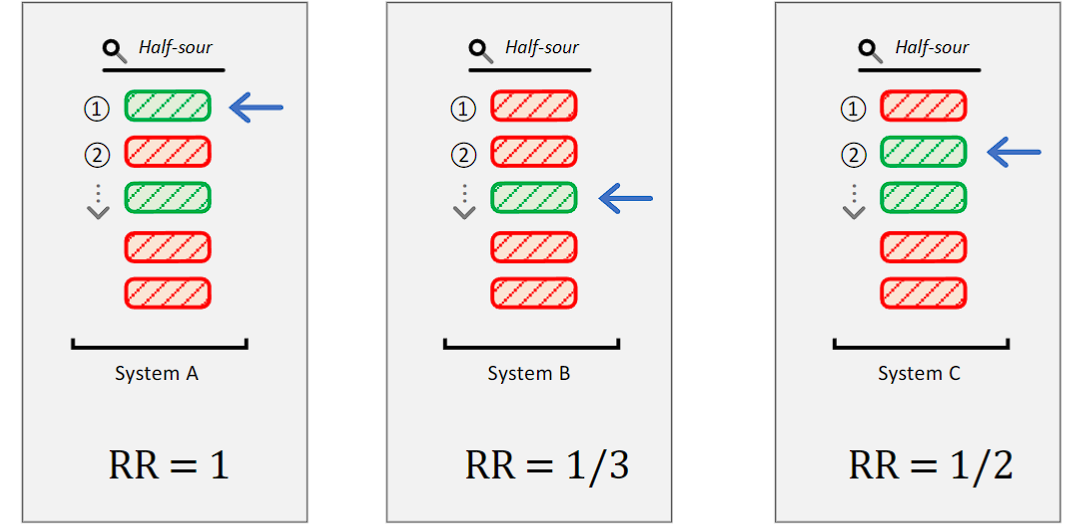
\includegraphics[width=1\textwidth]{assets/pics/rr.png}
        \caption{Ilustrasi \f{reciprocal rank}.}
        \label{fig:reciprocal-rank}
    \end{figure}
\end{frame}

\begin{frame}
    \frametitle{\f{Normalized Discounted Cumulative Gain}}
    \f{Normalized Discounted Cumulative Gain} (NDCG) adalah metrik yang umumnya digunakan untuk mengukur kualitas dari pencarian situs web. Tidak seperti metrik yang telah disebutkan sebelumnya, nDCG dirancang untuk suatu $r$ yang tak biner.
    \begin{flalign*}
        \text{nDCG}(q, D_k)\text{@k} &= \frac{\text{DCG}(q, D_k)\text{@k}}{\text{DCG}(q, D_k^{\text{ideal}})\text{@k}} \in [0, 1], && \\
        \text{DCG}(q, D_k)\text{@k} &= \sum_{d \in D_k} \frac{2^{\text{rel}(q, d)} - 1}{\log_2(\text{rank}(d, D_k) + 1)}, && \\
        \text{rank}(d,D_k) &= \text{Posisi } d \text{ dalam } D_k, && \\
        \text{rel}(q, d) &= r. &&
    \end{flalign*}  

\end{frame}

\begin{frame}
    \frametitle{\f{Normalized Discounted Cumulative Gain}}
    \begin{figure}[!ht]
        \centering
        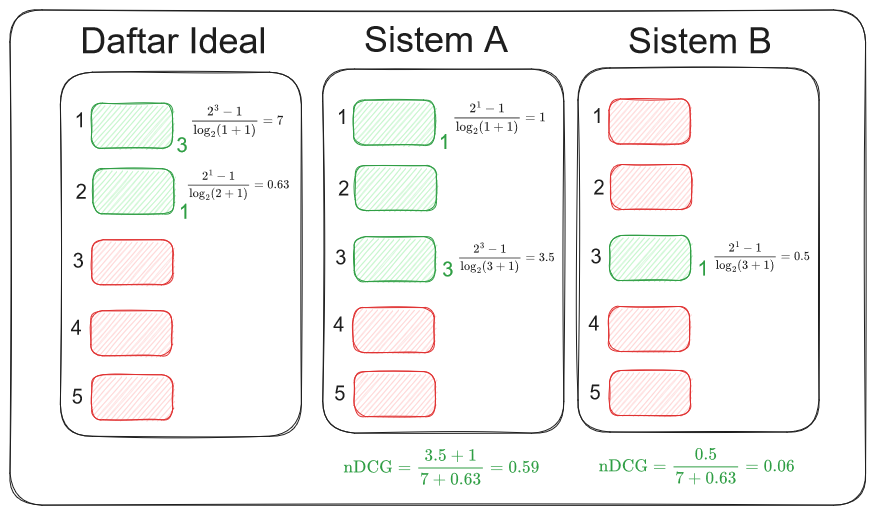
\includegraphics[width=1\textwidth]{assets/pics/contohnDCG.png}
        \caption{Ilustrasi \f{normalized discounted cumulative gain}.}
        \label{fig:ndcg}
    \end{figure}
\end{frame}

\section{Pemeringkatan Teks Dengan Statistik}

\begin{frame}
    \frametitle{{Pemeringkatan Teks Dengan Statistik}}

    \begin{enumerate}
        \item Untuk mengambil $k$ teks dari kumpulan $\mathcal{D}$, kita menggunakan fungsi skor $\text{score}(q, d, \mathcal{D})$ untuk mengukur relevansi antara kueri $q$ dan teks $d$. Dengan mencari skor antara $q$ dan semua teks pada $\mathcal{D}$, kita dapat memilih barisan teks $D_k = (d_{i_1}, d_{i_2},\dots, d_{i_k})$ dengan $k$ teks memiliki skor tertinggi.
        \item Salah satu fungsi skor mudah dan sering digunakan adalah TF-IDF dan BM25. Fungsi skor ini menghitung skor antara kueri $q$ dan teks $d$ dengan informasi dari kata yang ada pada $q$ dan $d$.
    \end{enumerate}
\end{frame}

\begin{frame}
    \frametitle{TF-IDF}
    \begin{itemize}
        \item \f{term frequency}: $\text{tf}(t, d) = \frac{\text{Count}(t, d)}{|d|}$,
        \item \f {document frequency}: $\text{df}(t, \mathcal{D}) = \text{jumlah teks pada } \mathcal{D} \text{ yang mengandung kata } t$. 
        \item \f{inverse document frequency}: $\text{idf}(t, \mathcal{D}) = \begin{cases}
            \log_2\left(\frac{|\mathcal{D}|}{\text{df}(t, \mathcal{D})}\right) & \text{jika } \text{df}(t, \mathcal{D}) > 0 \\
            0 & \text{jika } \text{df}(t, \mathcal{D}) = 0
        \end{cases}$.
        \item $\text{TF-IDF}(t, d, \mathcal{D}) = \text{tf}(t, d) \times \text{idf}(t, \mathcal{D})$.
    \end{itemize}

    \begin{figure}[!ht]
        \centering
        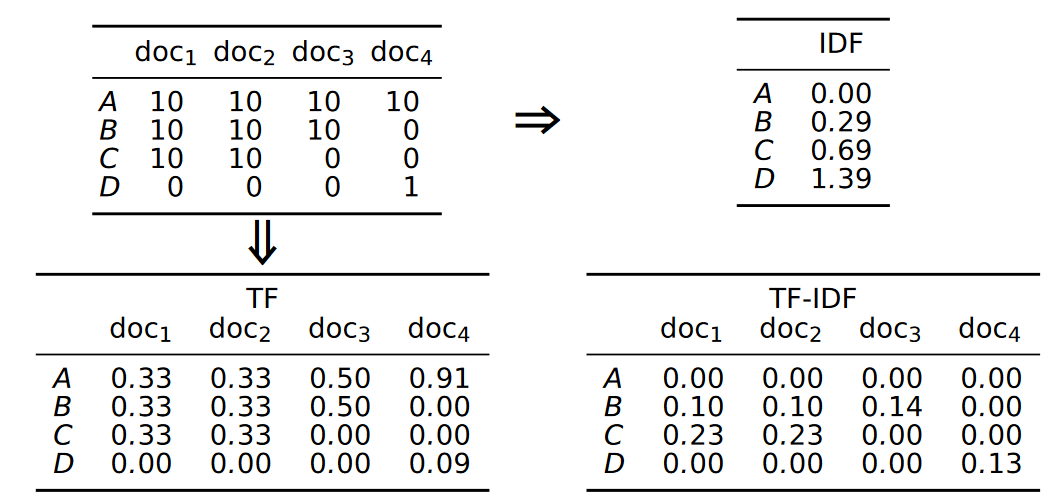
\includegraphics[width=1\textwidth]{assets/pics/tf-idf-matriks.png}
    \end{figure}
\end{frame}

\begin{frame}
    \frametitle{Nilai IDF}
    \begin{figure}[!ht]
        \centering
        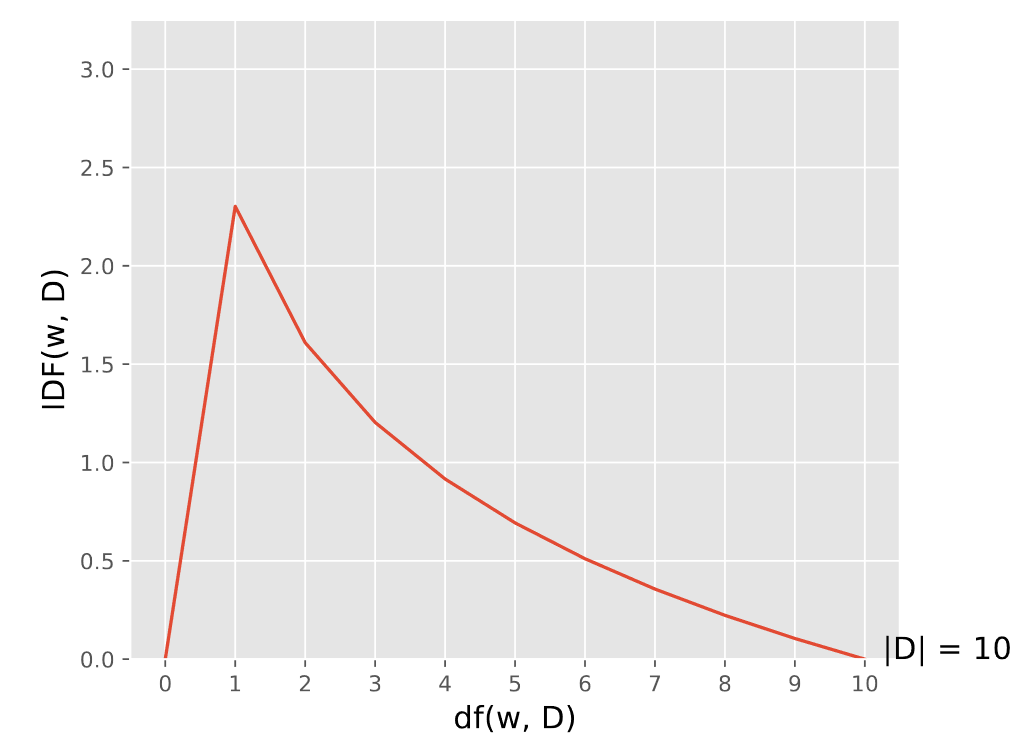
\includegraphics[width=1\textwidth]{assets/pics/idf-graph.png}
        \end{figure}
\end{frame}

\begin{frame}
    \frametitle{Score}
    $$\text{score}(q,d,\mathcal{D}) = \sum_{t \in T_q \cap T_d} \text{TF-IDF}(t, d, \mathcal{D})$$
    \begin{flalign*}
        T_q &= \{t_1, t_2, \dots, t_{L_1}\} = \text{kumpulan kata pada } q, && \\
        T_d &= \{t_1, t_2, \dots, t_{L_2}\} = \text{kumpulan kata pada } d. &&
    \end{flalign*}
\end{frame}

\begin{frame}
    \frametitle{BM25}

    \begin{block}{\f{Smoothed} IDF}
        $$
        \text{idf}_{\text{BM25}}(t, \mathcal{D}) = \log\left(1+\frac{|\mathcal{D}| - \text{df}(t, \mathcal{D}) + 0.5}{\text{df}(t, \mathcal{D}) + 0.5}\right)
        $$
    \end{block}

    \begin{block}{Score BM25 Pengganti tf}
        $$
        \text{score}_{\text{BM25}}(t,d) = \frac{\text{tf}(t, d) \times (k_1 + 1)}{\text{tf}(t, d) + k_1 \times (1 - b + b \times \frac{|d|}{\text{avgdl}})}
        $$
    \end{block}

    \begin{block}{BM25}
        $$
        \text{BM25}(t, d, \mathcal{D}) = \text{idf}_{\text{BM25}}(t, \mathcal{D}) \times \text{score}_{\text{BM25}}(q,d,\mathcal{D})
        $$
    \end{block}
    \cite{BM25ori}
\end{frame}



\section{Simulasi Dan Analisis Hasil}

\begin{frame}
    \frametitle{Dataset}
\end{frame}


\begin{frame}
    \frametitle{Dataset}

    Tabel berikut menunjukkan informasi mengenai jumlah entri dari \f{file} kueri, \f{file} korpus, dan \f{file jugdements} dari setiap \f{dataset} yang digunakan dalam penelitian ini.
    \begin{table}[!ht]
        \centering
        \begin{tabular}{|l|c|c|r|r|} \hline
            \textbf{Dataset} & \textbf{Korpus} & \textbf{Kueri} & \textbf{Jugdements} & \textbf{J/K} \\ \hline
            mMarco train set & 8,841,823       & 502,939        & 532,761             & 1.05                         \\ \hline
            mMarco dev set   & 8,841,823       & 6980           & 7,437               & 1.06                         \\ \hline
            Mrtydi test set  & 1,469,399       & 829            & 961                 & 1.15                        \\ \hline
            Miracl dev set   & 1,446,315       & 960            & 9,668               & 10.07                       \\ \hline
        \end{tabular}
    \end{table}    
\end{frame}

\begin{frame}
    \frametitle{Dataset}
    
    Tabel mengenai panjang kueri dan teks pada setiap \f{dataset}. \f{white space tokenizer} adalah \f{tokenizer} yang memisahkan teks menjadi kata-kata berdasarkan spasi. IndoBERT \f{tokenizer} adalah\f{tokenizer} yang digunakan pada model BERT yang digunakan pada penelitian ini.

    \begin{table}
        \footnotesize
        \begin{tabular}{lcccccccc}
            \multirow{2}{*}{Dataset} & \multicolumn{2}{c}{Min} & \multicolumn{2}{c}{Median} & \multicolumn{2}{c}{95\%th} & \multicolumn{2}{c}{Max} \\
            \cline{2-9}
            & Kueri & Teks & Kueri & Teks & Kueri & Teks & Kueri & Teks \\
            \multicolumn{9}{c}{IndoBERT \f{tokenizer}} \\
            \hline
            mMARCO \f{train set} & 3 & 3 & 9 & 62 & 14 & 123 & 247 & 772 \\
            mMARCO \f{dev set}   & 3 & 4 & 9 & 62 & 14 & 123 & 125 & 772 \\
            MrTyDI \f{test set}  & 6 & 3 & 9 & 48 & 13 & 172 & 23 & 6747 \\
            Miracl \f{dev set}   & 6 & 2 & 9 & 48 & 13 & 171 & 23 & 6747 \\
            \hline
            \multicolumn{9}{c}{\f{whitespace tokenizer}} \\
            mMARCO \f{train set} & 1 & 1 & 5 & 45 & 9 & 89 & 123 & 245 \\
            mMARCO \f{dev set}   & 1 & 1 & 5 & 45 & 10 & 89 & 31 & 245 \\
            MrTyDI \f{test set}  & 3 & 1 & 5 & 33 & 9 & 123 & 14 & 4462 \\
            Miracl \f{dev set}   & 3 & 1 & 5 & 33 & 8 & 123 & 14 & 4462 \\
            \hline
        \end{tabular}
    \end{table}
\end{frame}

\begin{frame}
    \frametitle{$\text{IndoBERT}_{\text{CAT}}$}
    \begin{enumerate}
        \item Arsitektur $\text{BERT}_\text{CAT}$ digunakan untuk melakukan pemeringkatan teks.
        \item Fungsi loss yang digunakan adalah \f{binary cross entropy}.
    \end{enumerate}

    \begin{align*}
        L(y, \hat{y}) &= - y_i \log(\hat{y}_i) - (1-y_i)\log(1-\hat{y}_i), \\
        \hat{y} &= P(\text{relevance} = 1 | q, d) = \sigma\left(  \mathbf{h}_{\text{[CLS]}} \mathbf{W}^{\text{CLS}}+\mathbf{b}^{\text{CLS}} \right) \in (0,1), \\
        \mathbf{h}_{\text{\code{[CLS]}}} &= \text{BERT}((\text{\code{[CLS]}}, q, \text{\code{[SEP]}}, d, \text{\code{[SEP]}}))_{\text{\code{[CLS]}}} \in \mathbb{R}^{d_{\text{token}}}, \\
        y &= \text{relevansi antara } q \text{ dan } d \in \{0, 1\}.
    \end{align*}

\end{frame}

\begin{frame}
    \frametitle{$\text{IndoBERT}_{\text{CAT}}$}
    Potongan \f{dataset} yang digunakan untuk pelatihan model $\text{IndoBERT}_{\text{CAT}}$.
    \begin{table}[!ht]
        \centering
        \small
        \begin{tabular}{|p{3cm}|p{4cm}|c|} \hline
            \textbf{Kueri}                                         & \textbf{Teks}                                                                                                                                                                                                                                                                                                                                                                                                                                                                                                                                                                                          & \textbf{Relevansi} \\ \hline
            Berapa banyak kalori sehari yang hilang saat menyusui? & Tidak hanya menyusui lebih baik untuk bayi, namun penelitian juga mengatakan itu lebih baik bagi ibu. Menyusui membakar rata-rata 500 kalori sehari, dengan kisaran khas antara 200 hingga 600 kalori yang terbakar sehari. Diperkirakan produksi 1 oz. $\dots$  & 1               \\ \hline
            Karakteristik iklim utama hutan hujan tropis           & Kacang kola adalah buah dari pohon kola, genus (Cola) pohon yang berasal dari hutan hujan tropis Afrika. & 0                  \\ \hline
        \end{tabular}
    \end{table}
    
\end{frame}


\begin{frame}
    \frametitle{ \f{hyperparameter}$\text{IndoBERT}_{\text{CAT}}$}
    \f{Hyperparameter} yang digunakan untuk \f{fine tuning }$\text{IndoBERT}_{\text{CAT}}$.
    \begin{table}[!ht]
        \centering
        \small
        \label{tab:indobert-cat-hyperparameter}
        \begin{tabular}{|c|c|}
            \hline
            \textbf{Parameter}       & \textbf{Nilai}                                                                                    \\
            \hline
            Model pralatih           & \href{https://huggingface.co/indolem/indobert-base-uncased}{\code{indolem/indobert-base-uncased}} \\
            \hline
            Total data               & 532,761                                                                                     \\
            \hline
            \f{Batch size}           & 32                                                                                                \\
            \hline
            Total iterasi            & 83243 (5 epochs)                                                                                  \\
            \hline
            \f{Optimizer}            & Adam dengan $\beta_1 = 0.9$, $\beta_2 = 0.999$, $\epsilon = 10^{-8}$                                 \\
            \hline
            \f{Learning rate}        & $2\times 10^{-5}$                                                                                              \\
            \hline
            \f{Learning rate warmup} & Linear selama 10\% dari total iterasi                                                             \\
            \hline
            Fungsi loss              & \f{Binary cross entropy}                                                                          \\
            \hline
        \end{tabular}
    \end{table}
    

\end{frame}

\begin{frame}
    \frametitle{$\text{IndoBERT}_{\text{DOT}}$}
    \begin{enumerate}
        \item Arsitektur $\text{BERT}_\text{DOT}$ digunakan untuk melakukan pemeringkatan teks.
        \item Fungsi loss yang digunakan adalah \f{N-pair loss}, dengan Teks negatif dipilih adalah teks positif untuk kueri lain pada \f{batch} yang sama \citep{dprmeta}.
    \end{enumerate}

    \begin{align*}
        L(q, d^+,\{d_i^-\}_{i=1}^{N-1}) = -\log \frac{\exp(\mathbf{h}^{\top}_q \mathbf{h}^+_d)}{\exp(\mathbf{h}^{\top}_q \mathbf{h}^+_d) + \sum_{i=1}^{N-1} \exp(\mathbf{h}^{\top}_q \mathbf{h}^-_i)},
    \end{align*}
    dengan keterangan sebagai berikut:
    \begin{flalign*}
        \mathbf{h}_q   &= \text{IndoBERT}_{\text{DOT}}((\code{[CLS]}, q, \code{[SEP]}))_{\code{[CLS]}} &&   \\
        \mathbf{h}^+_d &= \text{IndoBERT}_{\text{DOT}}((\code{[CLS]}, d^+, \code{[SEP]}))_{\code{[CLS]}} && \\
        \mathbf{h}^-_i &= \text{IndoBERT}_{\text{DOT}}((\code{[CLS]}, d^-_i, \code{[SEP]}))_{\code{[CLS]}} &&
    \end{flalign*}
    
\end{frame}

\begin{frame}
    \frametitle{$\text{IndoBERT}_{\text{DOT}}$}
    Ilustrasi fungsi objektif \f{N-pair loss}. Untuk pasangan teks yang relevan $(a, b_1)$, tujuannya adalah untuk meminimalkan jarak antara $a$ dan $b_1$ sehingga jarak tersebut lebih kecil dibandingkan dengan jarak antara $a$ dan $b_i$ yang lain.
    \begin{figure}[!ht]
        \centering
        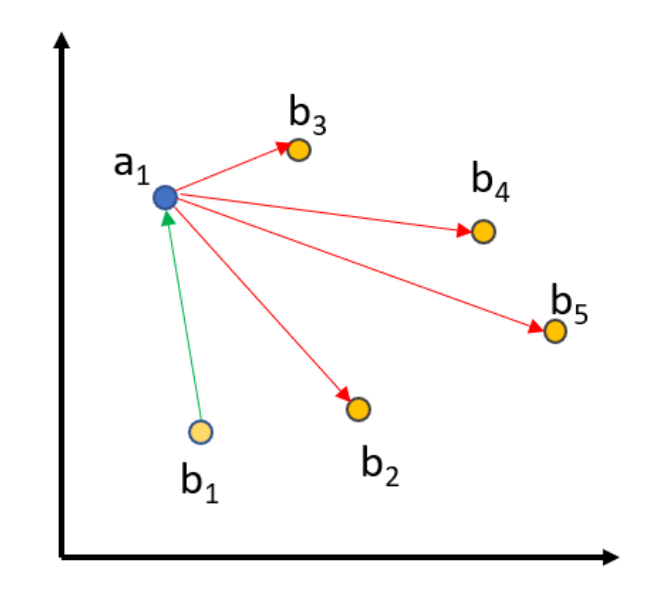
\includegraphics[width=0.5\textwidth]{assets/pics/InfoNCE.png}
    \end{figure}
    
\end{frame}

\begin{frame}
    \frametitle{\f{hyperparameter} $\text{IndoBERT}_{\text{DOT}}$}
    \f{Hyperparameter} yang digunakan untuk \f{fine tuning }$\text{IndoBERT}_{\text{DOT}}$.
    \begin{table}[!ht]
        \centering
        \small        
        \label{tab:indobert-dot-hyperparameter}
        \begin{tabular}{|c|c|}
            \hline
            \textbf{Parameter}       & \textbf{Nilai}                                                                                    \\
            \hline
            Model pralatih           & \href{https://huggingface.co/indolem/indobert-base-uncased}{\code{indolem/indobert-base-uncased}} \\
            \hline
            Total data               & 532,761                                                                                           \\
            \hline
            \f{Batch size}           & 32                                                                                                \\
            \hline
            Total iterasi            & 83,243 (5 epochs)                                                                                  \\
            \hline
            \f{Optimizer}            & Adam dengan $\beta_1 = 0.9$, $\beta_2 = 0.999$, $\epsilon = 10^{-8}$                                 \\
            \hline
            \f{Learning rate}        & $2\times 10^{-5}$                                                                                              \\
            \hline
            \f{Learning rate warmup} & Linear selama 10\% dari total iterasi                                                             \\
            \hline
            Fungsi \f{loss}          & \f{N-pair loss}                                                                                   \\
            \hline
        \end{tabular}
    \end{table}

    
\end{frame}


\begin{frame}
    \frametitle{$\text{IndoBERT}_{\text{DOThardnegs}}$}
    \begin{enumerate}
        \item Arsitektur $\text{BERT}_\text{DOT}$ digunakan untuk melakukan pemeringkatan teks.
        \item Fungsi loss yang digunakan adalah \f{N-pair loss}, dengan Teks negatif dipilih terlebih dahulu yang merupakan Teks yang serupa dengan teks positif namun tidak relevan dengan kueri.
    \end{enumerate}
\end{frame}

\begin{frame}
    \frametitle{$\text{IndoBERT}_{\text{DOThardnegs}}$}
    Potongan \f{file hard negative}. Kolom qid berisikan id dari kueri, kolom \f{positive} adalah id teks positif, dan kolom \f{hard negative} adalah id teks yang sulit dibedakan dengan teks positif.
    \begin{table}[!ht]
        \centering
        \small
        \label{tab:hardnegsbm25}
        \begin{tabular}{|c|c|p{8cm}|}
            \hline
            \bo{qid} & \bo{\f{Positive}} & \bo{\f{Hard Negative}}                                           \\
            \hline
            1185869 &  0  & [ 2942572, 5154062, 2942571, 5154065, 3870084 ] \\
            \hline
            1185868 &  16  & [ 6821177, 1641650, 1641656, 1641659, 1203539 ] \\
            \hline
            597651 &  49  & [ 6398884, 162755, 1838949, 1391482, 7818305 ] \\
            \hline
        \end{tabular}
    \end{table}
\end{frame}

\begin{frame}
    \frametitle{\f{hyperparameter} $\text{IndoBERT}_{\text{DOThardnegs}}$}
    \f{Hyperparameter} yang digunakan untuk \f{fine tuning }$\text{IndoBERT}_{\text{DOThardnegs}}$.
    \begin{table}[!ht]
        \centering
        \small

        \label{tab:indobert-dothardnegs-hyperparameter}
        \begin{tabular}{|c|c|}
            \hline
            \textbf{Parameter}       & \textbf{Nilai}                                                                                    \\
            \hline
            Model pralatih           & \href{https://huggingface.co/indolem/indobert-base-uncased}{\code{indolem/indobert-base-uncased}} \\
            \hline
            Total data               & 502,939                                                                                           \\
            \hline
            \f{Batch Size}           & 32                                                                                                \\
            \hline
            Total Iterasi            & 78585 (5 epochs)                                                                                  \\
            \hline
            \f{Optimizer}            & Adam dengan $\beta_1 = 0.9$, $\beta_2 = 0.999$, $\epsilon = 10^{-8}$                                 \\
            \hline
            \f{Learning rate}        & $2\times 10^{-5}$                                                                                              \\
            \hline
            \f{Learning rate warmup} & Linear selama 10\% dari total iterasi                                                             \\
            \hline
            Fungsi \f{loss}          & \f{N-pair loss}                                                                                   \\
            \hline
        \end{tabular}
    \end{table}    
\end{frame}

\begin{frame}
    \frametitle{$\text{IndoBERT}_{\text{DOTKD}}$}
    \begin{enumerate}
        \item Arsitektur $\text{BERT}_\text{DOT}$ digunakan untuk melakukan pemeringkatan teks.
        \item Fungsi loss yang digunakan adalah \f{Mean squared error} dengan prinsip \f{knowledge distillation} \citep{knowledgedistill}.
    \end{enumerate}
    \begin{align}
        L(s_i, t_i) = \left((\mid \mid M(s_i) - \hat{M}(s_i) \mid \mid)^2 + (\mid\mid M(s_i) - \hat{M}(t_i) \mid\mid)^2 \right),
    \end{align}
    dengan keterangan sebagai berikut:
    \begin{flalign*}
        M        &= \text{pemetaan vektor oleh model guru},&& \\
        \hat{M}  &= \text{pemetaan vektor oleh model murid},&& \\
        s_i      &= \text{teks sumber (bahasa Inggris)},&& \\
        t_i      &= \text{teks target (bahasa Indonesia)}.&&
    \end{flalign*}
\end{frame}

\begin{frame}
    \frametitle{$\text{IndoBERT}_{\text{DOTKD}}$}
    Ilustrasi dari pelatihan model $\text{IndoBERT}_{\text{DOTKD}}$ dengan \f{knowledge distillation}. Kalimat paralel diberikan sebagai \f{input}  pada model guru dan model murid. vektor yang dihasilkan oleh model guru dan model murid di-\f{align} menggunakan fungsi \f{loss mean squared error}.
    \begin{figure}[!ht]
        \centering
        \includegraphics[width=1\textwidth]{assets/pics/kd.png}
    \end{figure}
\end{frame}

\begin{frame}
    \frametitle{$\text{IndoBERT}_{\text{DOTKD}}$}
    Potongan dari \f{dataset} yang digunakan untuk pelatihan model $\text{IndoBERT}_{\text{KD}}$.
    \begin{table}[!ht]
        \centering
        \small
        \begin{tabular}{|p{4cm}|p{4cm}|}
            \hline
            \textbf{text\_en} & \textbf{txt\_id} \\
            \hline
            \f{Defining alcoholism as a disease is associated with Jellinek} & Mendefinisikan alkoholisme sebagai penyakit dikaitkan dengan Jellinek \\
            \hline
            \f{ECT is a treatment that is used for} & ECT adalah pengobatan yang digunakan untuk \\
            \hline
            \f{Ebolavirus is an enveloped virus, which means} & Ebolavirus adalah virus yang diselimuti, yang berarti \\
            \hline
            \f{How much does Cambridge Manor cost per month} & Berapa biaya Cambridge Manor per bulan? \\
            \hline
        \end{tabular}
    \end{table}
\end{frame}

\begin{frame}
    \frametitle{\f{hyperparameter} $\text{IndoBERT}_{\text{DOTKD}}$}
    \f{Hyperparameter} yang digunakan untuk \f{fine tuning }$\text{IndoBERT}_{\text{DOTKD}}$.
    \begin{table}[!ht]
        \centering
        \small
        \label{tab:indobert-kd-hyperparameter}
        \begin{tabular}{|c|c|}
            \hline
            \textbf{Parameter}       & \textbf{Nilai}                                                                                    \\
            \hline
            Model guru              & \href{https://huggingface.co/sentence-transformers/msmarco-bert-base-dot-v5}{\code{sentence-transformers/msmarco-bert-base-dot-v5}} \\
            \hline
            Model murid           & \href{https://huggingface.co/bert-base-multilingual-uncased}{\code{bert-base-multilingual-uncased}} \\
            \hline
            Total data               & 1,000,000                                                                                           \\
            \hline
            \f{Batch Size}           & 64                                                                                                \\
            \hline
            Total Iterasi            & 78125 (5 epochs)                                                                                  \\
            \hline
            \f{Optimizer}            & Adam dengan $\beta_1 = 0.9$, $\beta_2 = 0.999$, $\epsilon = 10^{-8}$                                 \\
            \hline
            \f{Learning rate}        & $2\times 10^{-5}$ \\
            \hline
            \f{Learning rate warmup} & Linear selama 10\% dari total iterasi                                                             \\
            \hline
            Fungsi \f{loss}          & \f{Mean squared error}                                                                            \\
            \hline
        \end{tabular}
    \end{table}
\end{frame}

\begin{frame}
\frametitle{Evaluasi Model}
\begin{enumerate}
    \item Setiap model dibandingkan dengan model baseline BM25.
    \item Implementasi BM25 menggunakan software ElasticSearch dengan parameter default, $b = 0.75$ dan $k_1 = 1.2$.
    \item \f{Stemming}, \f{lemmatization}, dan \f{stopword removal} diserahkan kepada ElasticSearch.
\end{enumerate}
\end{frame}

\begin{frame}
    \frametitle{Evaluasi Model $\text{IndoBERT}_{\text{CAT}}$}
    Evaluasi model $\text{IndoBERT}_{\text{CAT}}$ pada \f{dataset} mMarco \f{dev set}, MrTyDi \f{test set}, dan Miracl \f{dev set}. Catatan: tulisan bercetak tebal menunjukkan nilai tertinggi pada setiap kolom.
    \begin{table}[!ht]
        \centering
        \footnotesize
        \label{tab:indobertcat-hasil}
        \begin{tabular}{|c|c|c|c|c|c|c|} \hline
            Model                             & \multicolumn{2}{c|}{mMarco Dev} &
            \multicolumn{2}{c|}{MrTyDi Test} & \multicolumn{2}{c|}{Miracl Dev}                                             \\ \hline
                                              & RR@10 & R@100 & RR@10 & R@100 & NDCG@10 & R@100 \\ \hline
            BM25                              & .114  & .447   & .279   & .723   & \bo{.391}    & 811 \\ \hline
            BM25+$\text{IndoBERT}_{\text{CAT}}$    & \bo{.177}  & \bo{.568}   & \bo{.363}   & \bo{.830}   & .367    & \bo{853} \\ \hline
        \end{tabular}
    \end{table}
\end{frame}

\begin{frame}
    Evaluasi model $\text{IndoBERT}_{\text{DOT}}$ pada \f{dataset} mMarco \f{dev set}, MrTyDi \f{test set}, dan Miracl \f{dev set}. Catatan: tulisan bercetak tebal menunjukkan nilai tertinggi pada setiap kolom.
    \begin{table}[!ht]
    \centering
    \footnotesize
    \begin{tabular}
        {|c|c|c|c|c|c|c|} \hline
        Model                             & \multicolumn{2}{c|}{mMarco Dev} &
        \multicolumn{2}{c|}{MrTyDi Test} & \multicolumn{2}{c|}{Miracl Dev}                                             \\ \hline
                                          & RR@10 & R@100 & RR@10 & R@100 & NDCG@10 & R@100 \\ \hline
        BM25                              & .114  & .447   & .279   & .723   & \bo{.391}    & .\bo{.811} \\ \hline
        $\text{IndoBERT}_{\text{DOT}}$    & \bo{.181}  & \bo{.650}   & \bo{.324}   & \bo{.852}   & .319    & .741 \\ \hline
        
    \end{tabular}
\end{table}
\end{frame}

\begin{frame}
    \frametitle{Evaluasi Model $\text{IndoBERT}_{\text{DOThardnegs}}$}
    Evaluasi model $\text{IndoBERT}_{\text{DOThardnegs}}$ pada \f{dataset} mMarco \f{dev set}, MrTyDi \f{test set}, dan Miracl \f{dev set}. Catatan: tulisan bercetak tebal menunjukkan nilai tertinggi pada 
    \begin{table}[!ht]
        \centering
        \footnotesize
        \begin{tabular}{|c|c|c|c|c|c|c|} \hline
            Model                                     & \multicolumn{2}{c|}{mMarco Dev} &
            \multicolumn{2}{c|}{MrTyDi Test}          & \multicolumn{2}{c|}{Miracl Dev}                                             \\ \hline
                                                      & RR@10 & R@100 & RR@10 & R@100 & NDCG@10 & R@100 \\ \hline
                    BM25                              & .114  & .447   & .279   & .723   & .391    & \bo{.811} \\ \hline
            $\text{IndoBERT}_{\text{DOThardnegs}}$    & \bo{.232}  & \bo{.680}   & \bo{.471}   & \bo{.824}   & \bo{.397}    & .726 \\ \hline
        \end{tabular}
    \end{table}    
\end{frame}

\begin{frame}
    \frametitle{Evaluasi Model $\text{IndoBERT}_{\text{DOTKD}}$}
    Evaluasi model $\text{IndoBERT}_{\text{DOTKD}}$ pada \f{dataset} mMarco \f{dev set}, MrTyDi \f{test set}, dan Miracl \f{dev set}. Catatan: tulisan bercetak tebal menunjukkan nilai tertinggi pada setiap kolom.
    \begin{table}[!ht]
        \centering
        \footnotesize
        \begin{tabular}{|c|c|c|c|c|c|c|} \hline
            Model                             & \multicolumn{2}{c|}{mMarco Dev} &
            \multicolumn{2}{c|}{MrTyDi Test} & \multicolumn{2}{c|}{Miracl Dev}                                             \\ \hline
                                              & RR@10 & R@100 & RR@10 & R@1000 & NDCG@10 & R@1000 \\ \hline
            BM25                              & .114  & .447   & .279   & .723   & .391    & .811 \\ \hline
            $\text{IndoBERT}_{\text{DOTKD}}$  & \bo{.235}  & \bo{.705}   & .393   & .751   & .374    & .702    \\ \hline
        \end{tabular}
    \end{table}
\end{frame}

\begin{frame}
    \frametitle{Evaluasi Model}
    Evaluasi dari model $\text{IndoBERT}_{\text{CAT}}$, $\text{IndoBERT}_{\text{DOT}}$, $\text{IndoBERT}_{\text{DOThardnegs}}$, dan $\text{IndoBERT}_{\text{DOTKD}}$ pada \f{dataset} mMarco \f{dev set}, MrTyDi \f{test set}, dan Miracl \f{dev set}.
    \begin{table}[!ht]
        \centering
        \footnotesize
        \label{tab:evaluasisemuamodel}
        \begin{tabular}{|c|c|c|c|c|c|c|} \hline
            Model                             & \multicolumn{2}{c|}{mMarco Dev} &
            \multicolumn{2}{c|}{MrTyDi Test} & \multicolumn{2}{c|}{Miracl Dev}                                             \\ \hline
                                              & RR@10 & R@100 & RR@10 & R@100 & NDCG@10 & R@100 \\ \hline
            BM25                              & .114  & .447   & .279   & .723   & .391    & .811 \\ \hline
            BM25+$\text{IndoBERT}_{\text{CAT}}$    & .177  & .568   & .363   & .830   & .367    & \bo{.853} \\ \hline
            $\text{IndoBERT}_{\text{DOT}}$    & .181  & .650   & .324   & \bo{.852}   & .319    & .741 \\ \hline
            $\text{IndoBERT}_{\text{DOThardnegs}}$    & .232  & .680   & \bo{.471}   & .824   & \bo{.397}    & .726 \\ \hline
            $\text{IndoBERT}_{\text{DOTKD}}$  & \bo{.235}  & \bo{.705}   & .393   & .751   & .374    & .702    \\ \hline
        \end{tabular}
    \end{table}
\end{frame}


\section{Penutup}

\begin{frame}
    \frametitle{Kesimpulan}
    \begin{enumerate}
        \item  Berdasarkan penjelasan dan implementasi pada presentasi telah ditunjukkan dua cara penggunaan BERT untuk pemeringakatan teks, yaitu BERT sebagai \f{soft classifier} dari nilai relevansi (kueri, teks) dan BERT sebagai pemetaan teks ke dalam ruang vektor dengan nilai skor relevansi dihitung dengan fungsi \f{similarity} seperti jarak kosinus dan \f{dot product}.
        \item tabel pada slide sebelumnya, telah ditunjukkan bahwa model BERT yang dilatih kembali (\f{fine tuning}) pada \f{dataset} Mmarco \f{train set} menghasilkan skor yang lebih baik dibandingkan dengan model \f{baseline} BM25 pada dua \f{dataset} uji Mmarco \f{dev set} dan MrTyDi \f{dev set}. Pada \f{dataset} Miracl \f{dev set}, hanya $\text{IndoBERT}_{\text{DOThardnegs}}$ yang menghasilkan skor yang lebih baik dibandingkan dengan model \f{baseline} BM25 pada metrik NDCG@10. dan $\text{IndoBERT}_{\text{CAT}}$ yang menghasilkan skor yang lebih baik pada metrik R@100.
    \end{enumerate}
\end{frame}


\begin{frame}
    \frametitle{Saran}
    \begin{enumerate}
        \item Pelatihan model BERT dapat dilakukan dengan \f{dataset} yang lebih beragam. 
        \item Memperbanyak \f{dataset} uji untuk pemeringkatan teks, sehingga dapat dilakukan analisis yang lebih mendalam terhadap setiap model yang dihasilkan.
        \item Menambah jumlah model \f{baseline} untuk pemeringkatan teks. Beberapa model yang dapat ditambahkan adalah TF-IDF, Word2Vec, ELMo, dan arsitektur \f{non-transformer} seperti LSTM dan CNN.
    \end{enumerate}
    
\end{frame}

\begin{frame}[allowframebreaks]
    \frametitle{Daftar Pustaka}
    \bibliography{references}
\end{frame}

\end{document}